\chapter{Khảo sát dữ liệu và tiền xử lý dữ liệu}
\section{Các tập dữ liệu sử dụng}
Để mô hình xây dựng đủ độ chính xác và có tính ứng dụng thực tế cũng như có thể được đánh giá khách quan, chúng tôi sử dụng các tập dữ liệu thực 
\subsection{SLIVER07}
\subsection{3Dircadb}
\subsection{LITS2017}
\section{Tiền xử lý dữ liệu}
\subsection{Chuẩn hóa dữ liệu}
\paragraph{Hounsfield unit (HU)} Hounsfield unit (còn được gọi là số CT), được đặt theo tên Sir Godfrey Hounsfield,là thang đo định lượng mô tả mật độ phóng xạ trong ảnh chụp cắt lớp vi tính. Giá trị HU của không khí được định nghĩa -1000 HU và của nước là 0 HU.
\paragraph{Chuẩn hóa giá trị Hounsfield unit (HU)} Bao gồm các bước sau:
\begin{enumerate}
\item Đưa thang đo về khoảng [-1000, 400]: Thay đổi giá trị HU của những voxel có giá trị thấp hơn -1000 HU về -1000 HU, những voxel có giá trị cao hơn 400 HU về 400 HU
\item Đưa thang đo về khoảng [0, 1400]: Cộng 1000 (HU) vào giá trị mỗi voxel
\item Chuẩn hóa giá trị [0,1]: Chia giá trị mỗi voxel cho 1400
\end{enumerate}
Sau bước chuẩn hóa, giá trị trên mỗi voxel nằm trong khoảng [0,1] dạng 32-bit single-precision floating-point.

\begin{figure*}
  \centering
  \subfigure[Chưa thực hiện tiền xử lý]{%
    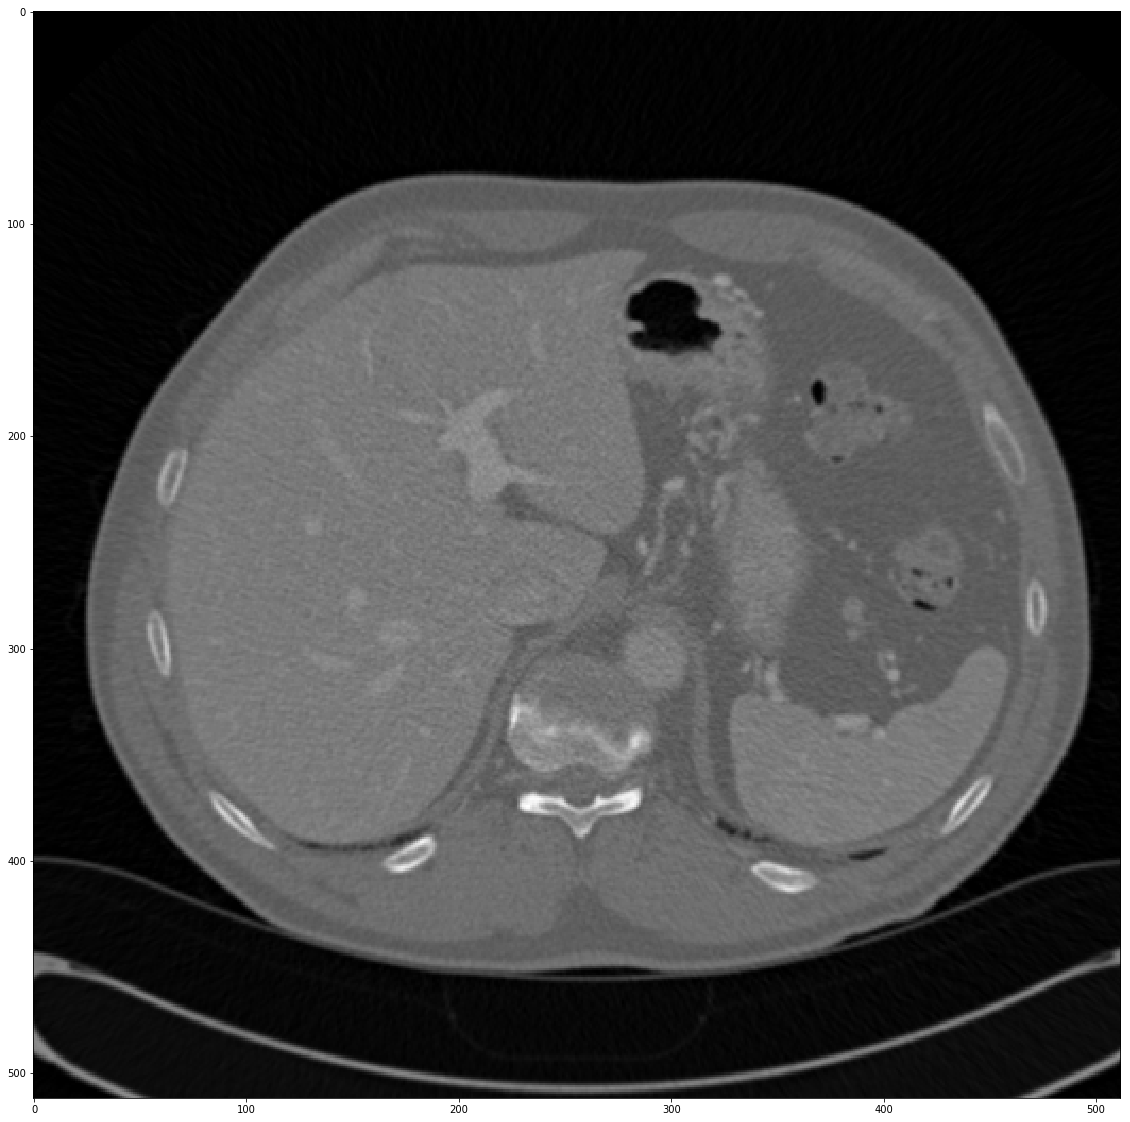
\includegraphics[width=0.3\textwidth]{Images/Liver_org.png}%
    \label{fig:image5}%
    }
    \subfigure[Sau khi chuẩn hóa.]{%
    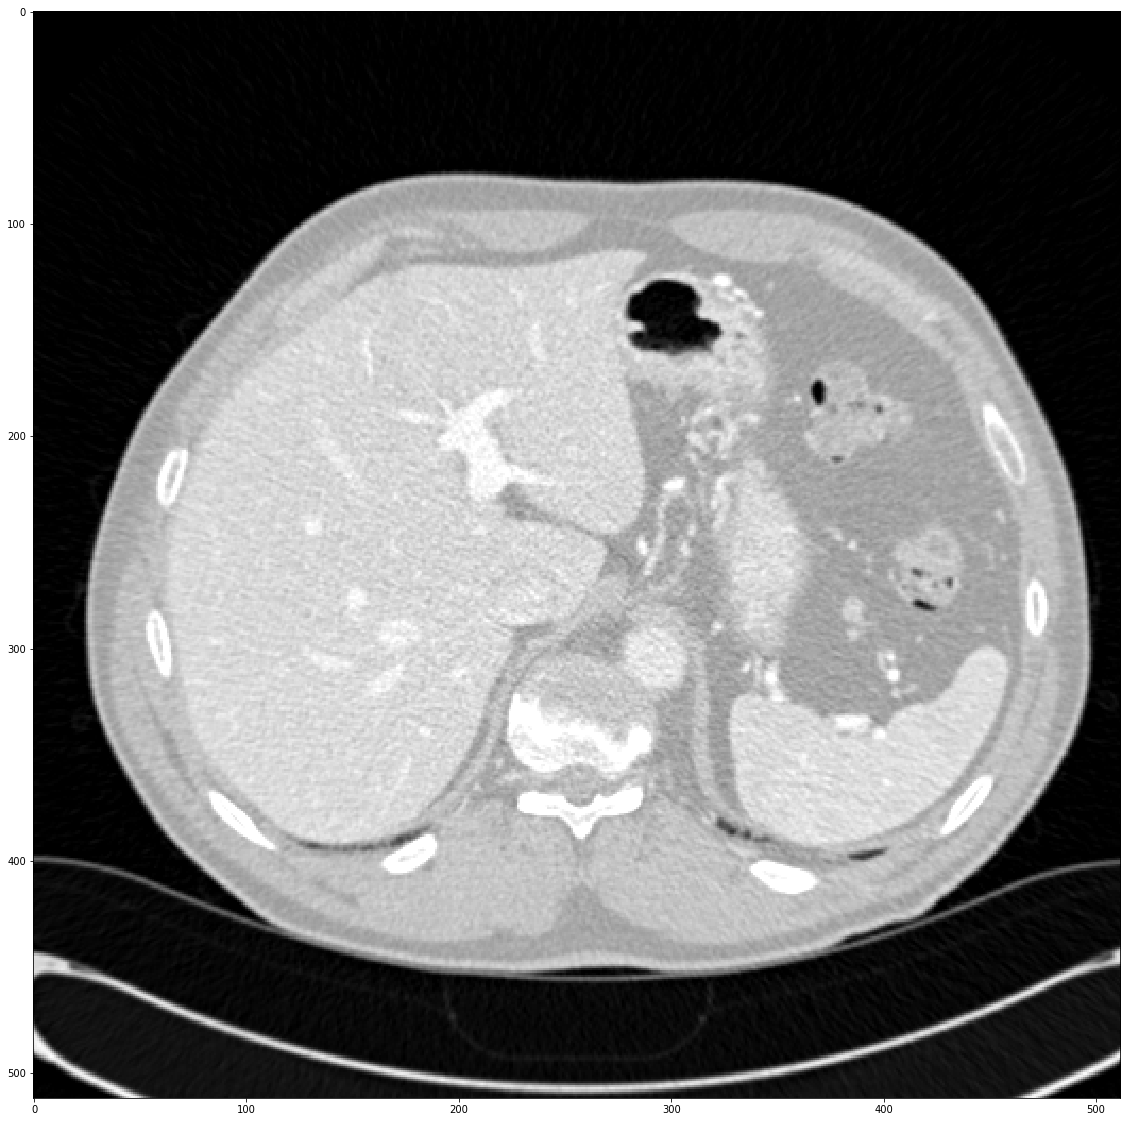
\includegraphics[width=0.3\textwidth]{Images/Liver_norm.png}%
    \label{fig:b}%
    }
    \subfigure[Đã loại bỏ nhiễu.]{%
    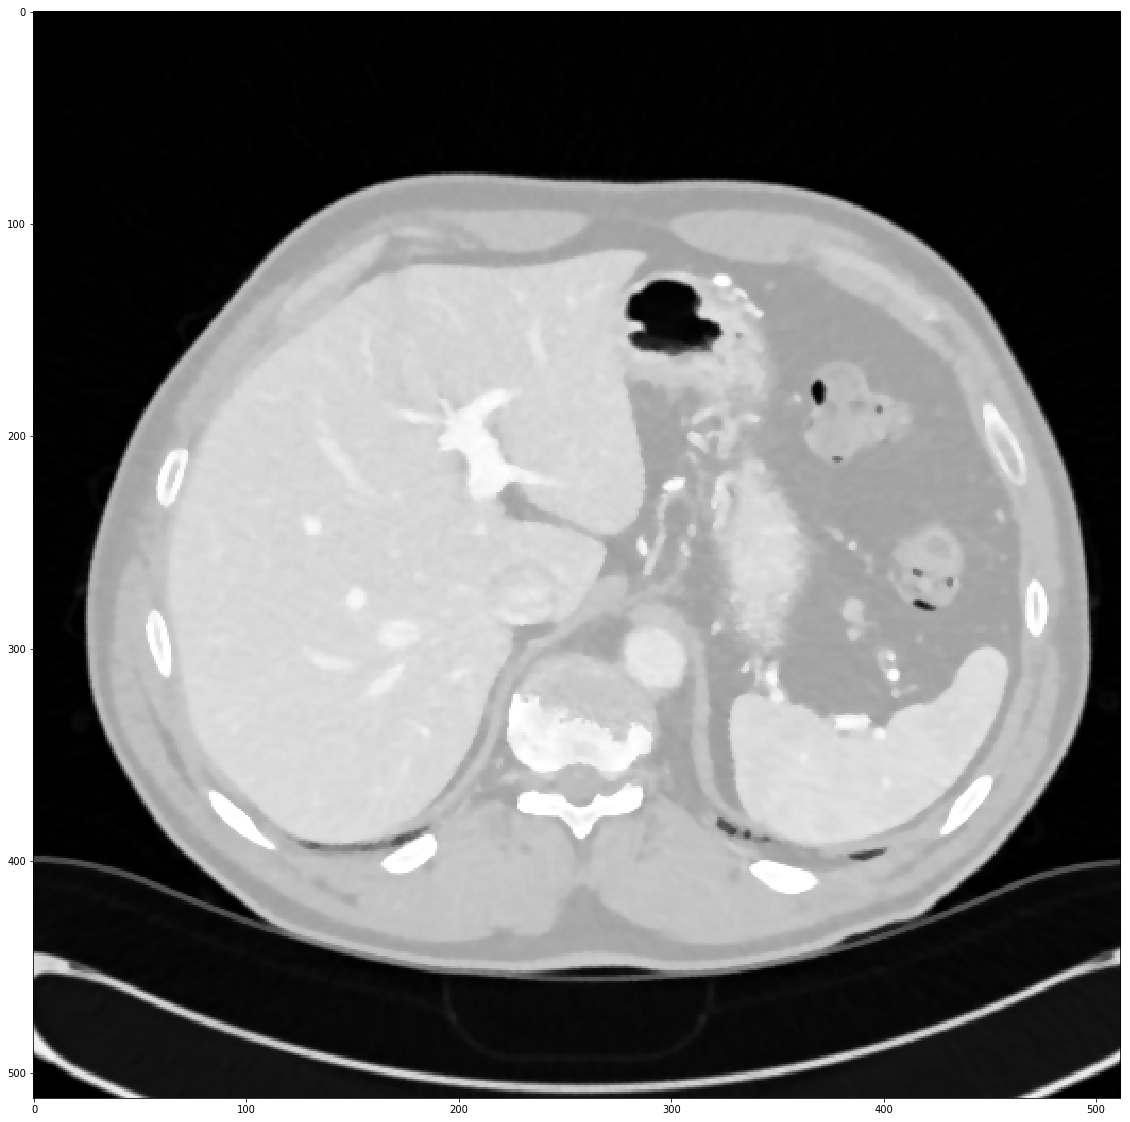
\includegraphics[width=0.3\textwidth]{Images/Liver_rm_noise.png}%
    \label{fig:c}%
    }% 
  \caption{Minh hoạ quá trình tiền xử lý một lát cắt trên ảnh CT}
  \label{fig:ab}
\end{figure*}

\subsection{Loại bỏ nhiễu}
Chúng tôi đã sử dụng công cụ Isotropic diffusion filter trong thư viện SimpleItk để loại bỏ nhiểu. Các tham số sử dụng:
\begin{itemize}
    \item Iterations: 10
    \item TimeStep: 0.625
    \item Conductance Parameter: 1.5
\end{itemize}
\subsection{Isometric}
Dữ liệu trên các tập SLIVER07, 3Dircadb và LITS2017 có khoảng cách giữa các voxel (spacing) rất khác nhau sẽ gây khó khăn cho mô hình phân đoạn. Đặc biệt là khoảng cách giữa các voxels trục Z ứng với khoảng cách giữa các lát cắt nằm trong khoảng rất lớn, từ 0.5 mm đến 6 mm. Vì vậy, chúng tôi đã đồng bộ khoảng cách giữa các voxels trên tất cả các trục về 1 (mm) đối với tất cả các mẫu dữ liệu. Việc này được thực hiện bằng công cụ Zoom trong thư viện Scipy với nội suy Cubic Spline, $Zoom = (Spacing_x, Spacing_y, Spacing_z)$.

